\section{Anhang}
\label{sec:Anhang}

\begin{figure}
    \centering
    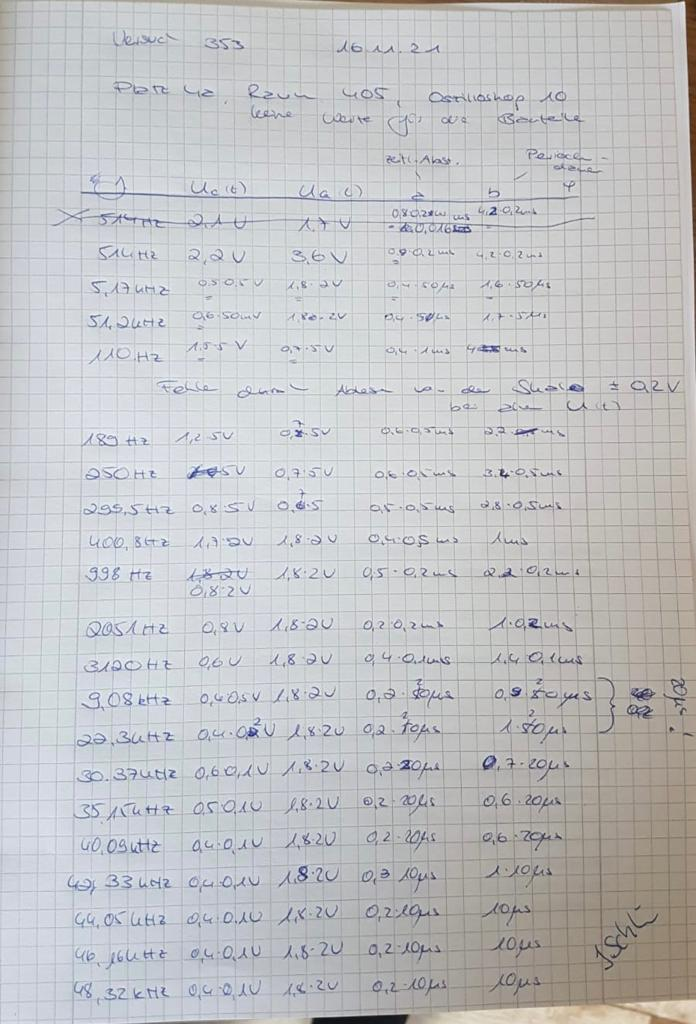
\includegraphics[scale=0.4]{content/origDaten.png}
    \caption{Die genommenen Originaldaten.}
    \label{fig:origDaten}
\end{figure}

\begin{table}
  \centering
  \caption{Die Tabelle mit allen vor Ort aufgenommenen Messdaten.}
  \label{tab:DatenAbgelesen}
  \begin{tabular}{
      S[table-format=2.4]
      S[table-format=1.2]
      S[table-format=1.1]
      S[table-format=3]
      S[table-format=4.1]
    }
      \toprule
      {$f \mathbin{/} \unit{\kilo\hertz}$} &
      {$U_c \mathbin{/} \unit{\volt}$} &
      {$U_G \mathbin{/} \unit{\volt}$} &
      {$a \mathbin{/} \unit{\micro\second}$} &
      {$b \mathbin{/} \unit{\micro\second}$} \\
      \midrule
      0.1100 & 7.50  & 3.5 & 400 & 4000.0 \\
      0.1890 & 6.00    & 3.5 & 300 & 2200.0 \\
      0.2500 & 5.00    & 3.5 & 300 & 1700.0 \\
      0.2995 & 4.00    & 3.5 & 250 & 1400.0 \\
      0.4008 & 3.40  & 3.6 & 200 & 1000.0 \\
      0.5140 & 2.20  & 3.6 & 160 & 840.0  \\
      0.9980 & 1.60  & 3.6 & 100 & 440.0  \\
      2.0510 & 0.80  & 3.6 & 40  & 200.0 \\
      3.1200 & 0.60  & 3.6 & 40  & 140.0  \\
      5.1700 & 0.25 & 3.6 & 20  & 80.0   \\
      9.0800 & 0.20  & 3.6 & 4   & 16.0   \\
      22.3400 & 0.08 & 3.6 & 4   & 20.0   \\
      30.3700 & 0.06 & 3.6 & 4   & 14.0   \\
      35.1500 & 0.05 & 3.6 & 4   & 12.0   \\
      40.0900 & 0.04 & 3.6 & 4   & 12.0   \\
      42.3300 & 0.04 & 3.6 & 2   & 10.0   \\
      44.0500 & 0.04 & 3.6 & 2   & 10.0   \\
      46.1600 & 0.04 & 3.6 & 2   & 10.0  \\
      48.3200 & 0.04 & 3.6 & 2   & 10.0   \\
      51.2400 & 0.03 & 3.6 & 2   & 8.5  \\
      \bottomrule
  \end{tabular}
\end{table}
